\documentclass[aspectratio=169, 8pt, xcolor={svgnames}, hyperref={linkcolor=black}]{beamer}
\usepackage[labelfont={color=amethyst,bf}]{caption}
\setbeamercolor{background canvas}{bg=white}
\usetheme[progressbar=frametitle]{metropolis}
\usepackage{appendixnumberbeamer}
\usepackage{url}
\usepackage{booktabs}
\usepackage{braket}
\usepackage[scale=2]{ccicons}
\usepackage{amsfonts} 
\usepackage{amssymb}
\usepackage[english]{babel}
\colorlet{col1}{teal}
\colorlet{col2}{yellow}
\colorlet{col3}{green}
\usepackage{fontawesome}
\usepackage{subcaption}
\usepackage{multicol}
\usepackage{bm}
\usepackage{algorithm}
\usepackage{overpic}
\usepackage{algpseudocode}
\usepackage{enumitem}

\usepackage[]{pseudo}


\usepackage{tikz}
\usetikzlibrary{positioning,arrows,calc,math,angles,quotes}
\usepackage{blochsphere}


\usetikzlibrary{arrows,automata}
\usetikzlibrary{positioning}
\usetikzlibrary{arrows.meta,
                bending,
                intersections,
                quotes,
                shapes.geometric}

\tikzset{
    state/.style={
           rectangle,
           rounded corners,
           draw=black, very thick,
           minimum height=1em,
           inner sep=2pt,
           text centered,
           },
}


\definecolor{myv}{rgb}{0.36, 0.22, 0.33}
\definecolor{gio}{rgb}{0.45, 0.31, 0.59}
\definecolor{light}{rgb}{0.8, 0.8, 1}
\definecolor{warmblack}{rgb}{0.0, 0.26, 0.26}
\definecolor{brown(web)}{rgb}{0.65, 0.16, 0.16}
\definecolor{cadmiumgreen}{rgb}{0.0, 0.42, 0.24}
\definecolor{darkmidnightblue}{rgb}{0.0, 0.2, 0.4}
\definecolor{brightube}{rgb}{0.82, 0.62, 0.91}

\definecolor{codegreen}{rgb}{0,0.6,0}
\definecolor{codegray}{rgb}{0.5,0.5,0.5}
\definecolor{codepurple}{rgb}{0.58,0,0.82}
\definecolor{backcolour}{rgb}{0.95,0.95,0.92}
\definecolor{amethyst}{rgb}{0.6, 0.33, 0.73}

\definecolor{light-gray}{gray}{0.95}
\newcommand{\code}[1]{\colorbox{light-gray}{\texttt{#1}}}


\usepackage{listings}
\lstdefinestyle{mystyle}{
    backgroundcolor=\color{backcolour},   
    commentstyle=\color{codegreen},
    keywordstyle=\color{codepurple},
    numberstyle=\tiny\color{codepurple},
    stringstyle=\color{magenta},
    basicstyle=\footnotesize,
    breakatwhitespace=false,         
    breaklines=true,                 
    captionpos=b,                    
    keepspaces=true,                 
    numbers=left,                    
    numbersep=5pt,                  
    showspaces=false,                
    showstringspaces=false,
    showtabs=false,                  
    tabsize=2
}

\lstset{style=mystyle}
\usepackage[most]{tcolorbox}
\usepackage{xcolor}


%\usepackage[citecolor = green, linkcolor = blue, bookmarks=true, urlcolor=blue,
%colorlinks=true, pagebackref=true]{hyperref}


%\usepackage{xspace}

\title{Grover search algorithm}
\subtitle{Quantum Computing Minicourse ICTP-SAIFR}
\date{8 April 2024}
\author{Stefano Carrazza$^\ddag$ and Matteo Robbiati$^\dagger$}
\institute{$^\ddag$ Associate Professor \& Researcher, University of Milan and INFN Milan, Italy.\\
$^\dagger$ PhD candidate, University of Milan, Italy and CERN, Switzerland.}
\titlegraphic{
\begin{tikzpicture}[overlay, remember picture]

\node[at=(current page.south), anchor=south, shift={(-3cm, 0)}] {%
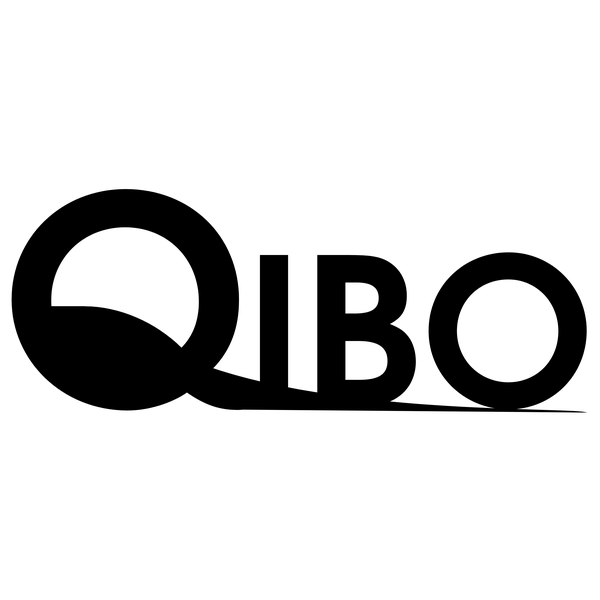
\includegraphics[width=.12\textwidth]{figures/qibo.png}

\includegraphics[width=.12\textwidth]{figures/unimi.png}

\includegraphics[width=.12\textwidth]{figures/cern.png}

\includegraphics[width=.12\textwidth]{figures/ictp.png}
};
\end{tikzpicture}
}


\begin{document}

\begin{frame}
\maketitle
\begin{picture}(0,0)
    \put(270,20){
        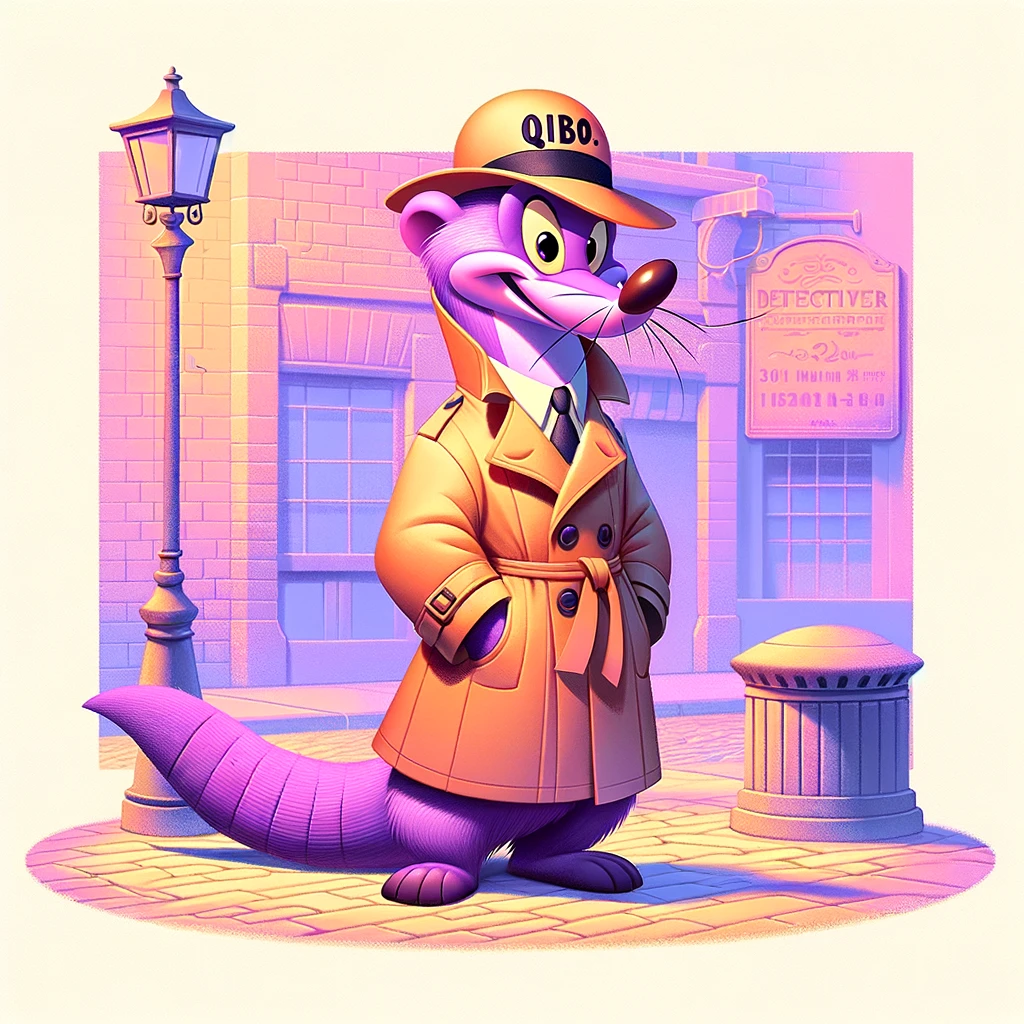
\includegraphics[width=0.3\textwidth]{figures/qibo_detective.png}
    }
\end{picture}
\end{frame}

\begin{frame}{Motivation}
The Grover algorithm is powerful when searching an item 
among an unordered set of candidates. 

\begin{multicols}{3}
Extract the jack of clubs from a Poker deck
\begin{figure}
    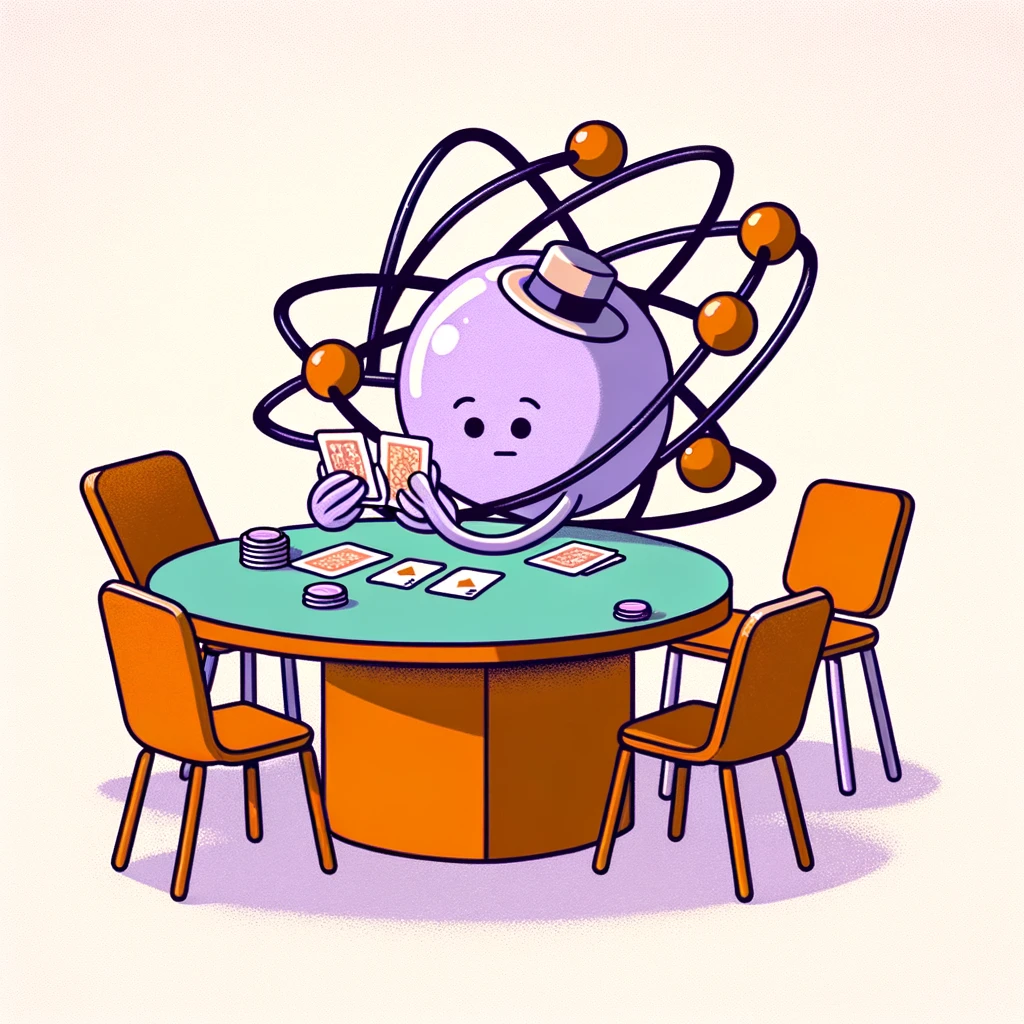
\includegraphics[width=.25\textwidth]{figures/poker.png}
\end{figure}

Find a passcode composed of 10 numbers
\begin{figure}
    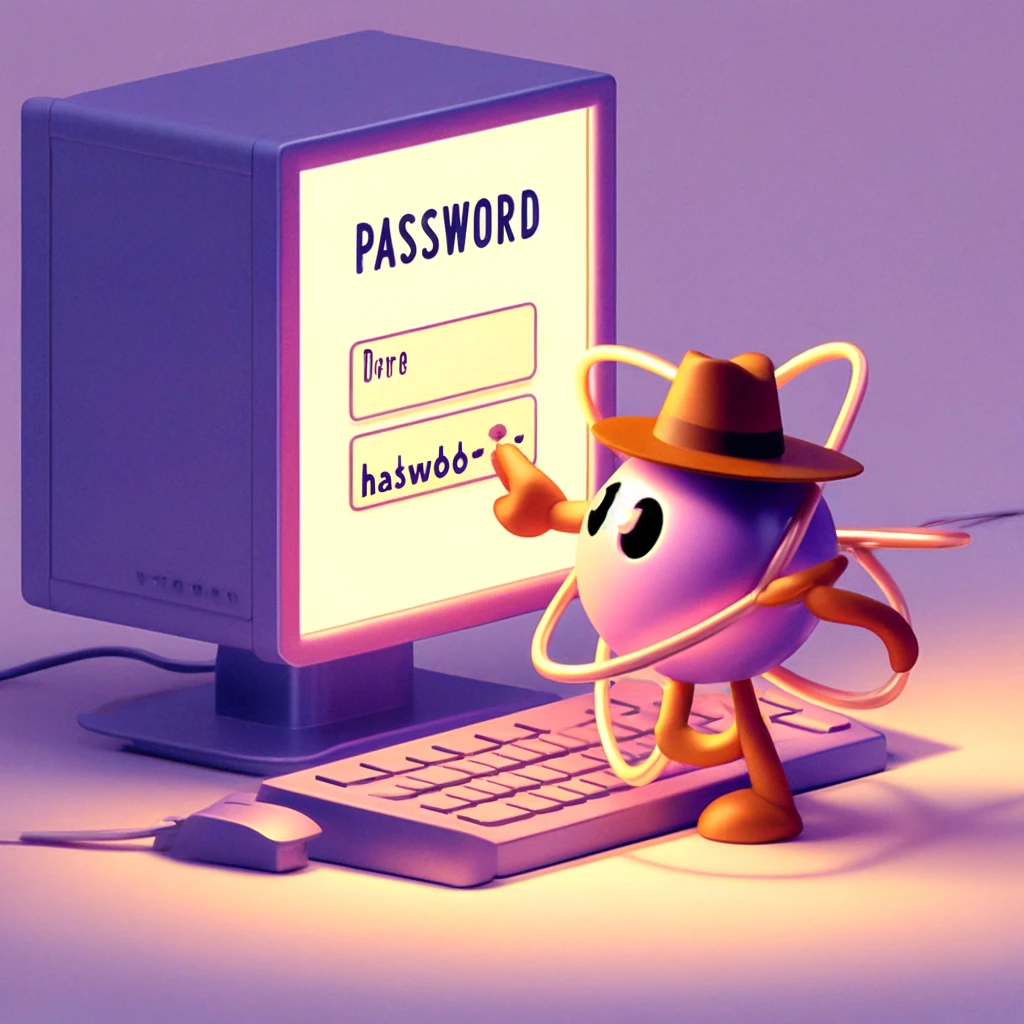
\includegraphics[width=.25\textwidth]{figures/pwd.png}
\end{figure}

Find an antidote to the Cobra poison, exploring $10^{20}$ 
molecules
\begin{figure}
    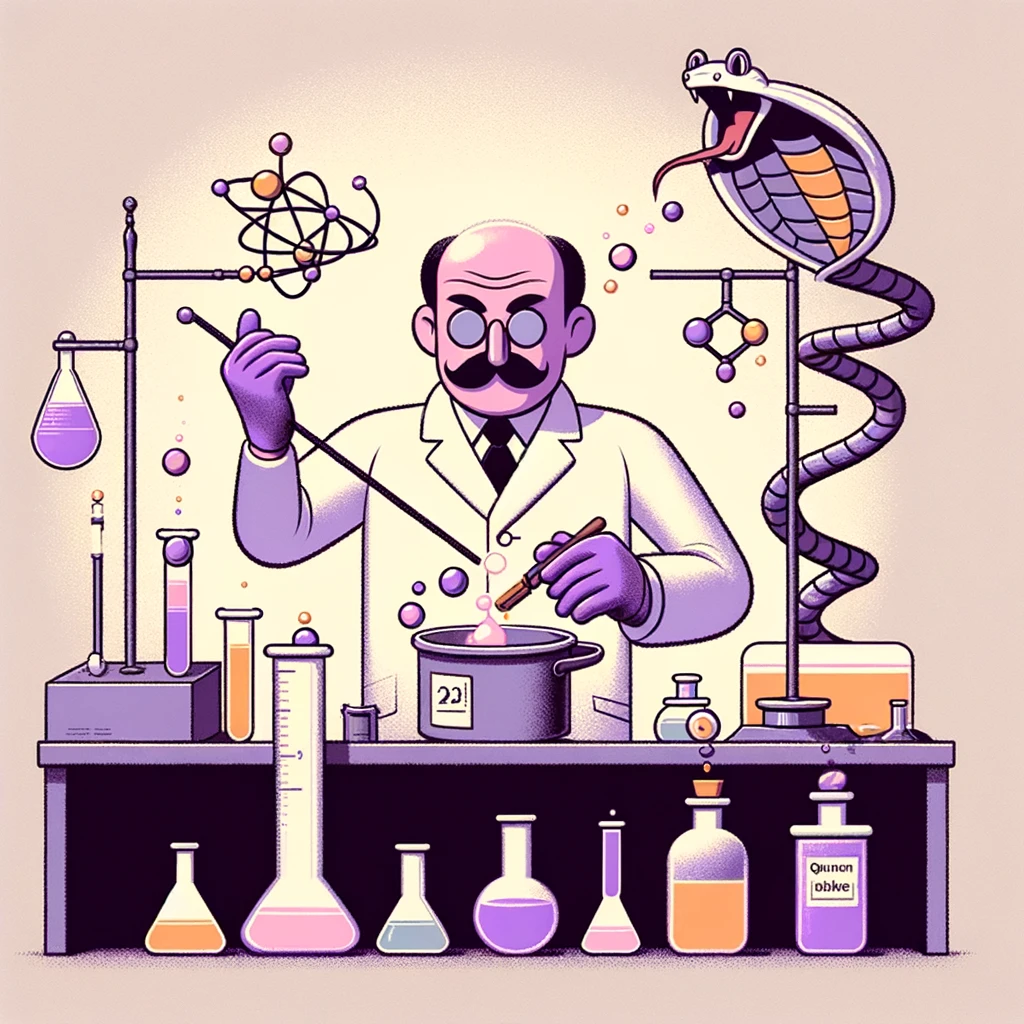
\includegraphics[width=.25\textwidth]{figures/cobra.png}
\end{figure}
\end{multicols}

\faQuestion\,\,How many attempts could you need, in the worst scenario, to explore all the possibilities?

\faExclamationTriangle\,\, In the worst scenario, you will need to check \textbf{$52$ cards}, \textbf{$10^{10}$} \textbf{passcodes}
and \textbf{$10^{20}$} \textbf{molecules}.
\end{frame}

\begin{frame}{Quadratic speedup}
If we consider a time cost of $\delta=10^{-8}$ seconds for any algorithmic call (quantum or classical) we would wait:
\begin{multicols}{2}
\textbf{On a classical computer}
\begin{itemize}[noitemsep]
\item[\footnotesize\faCircle] $0.52\,\,\mu \text{s}$ to find the jack of clubs;
\item[\footnotesize\faCircle] $100$ seconds to find the passcode;
\item[\footnotesize\faCircle] $\sim 31688$ years to find the Cobra antidote.
\end{itemize}
\begin{figure}
    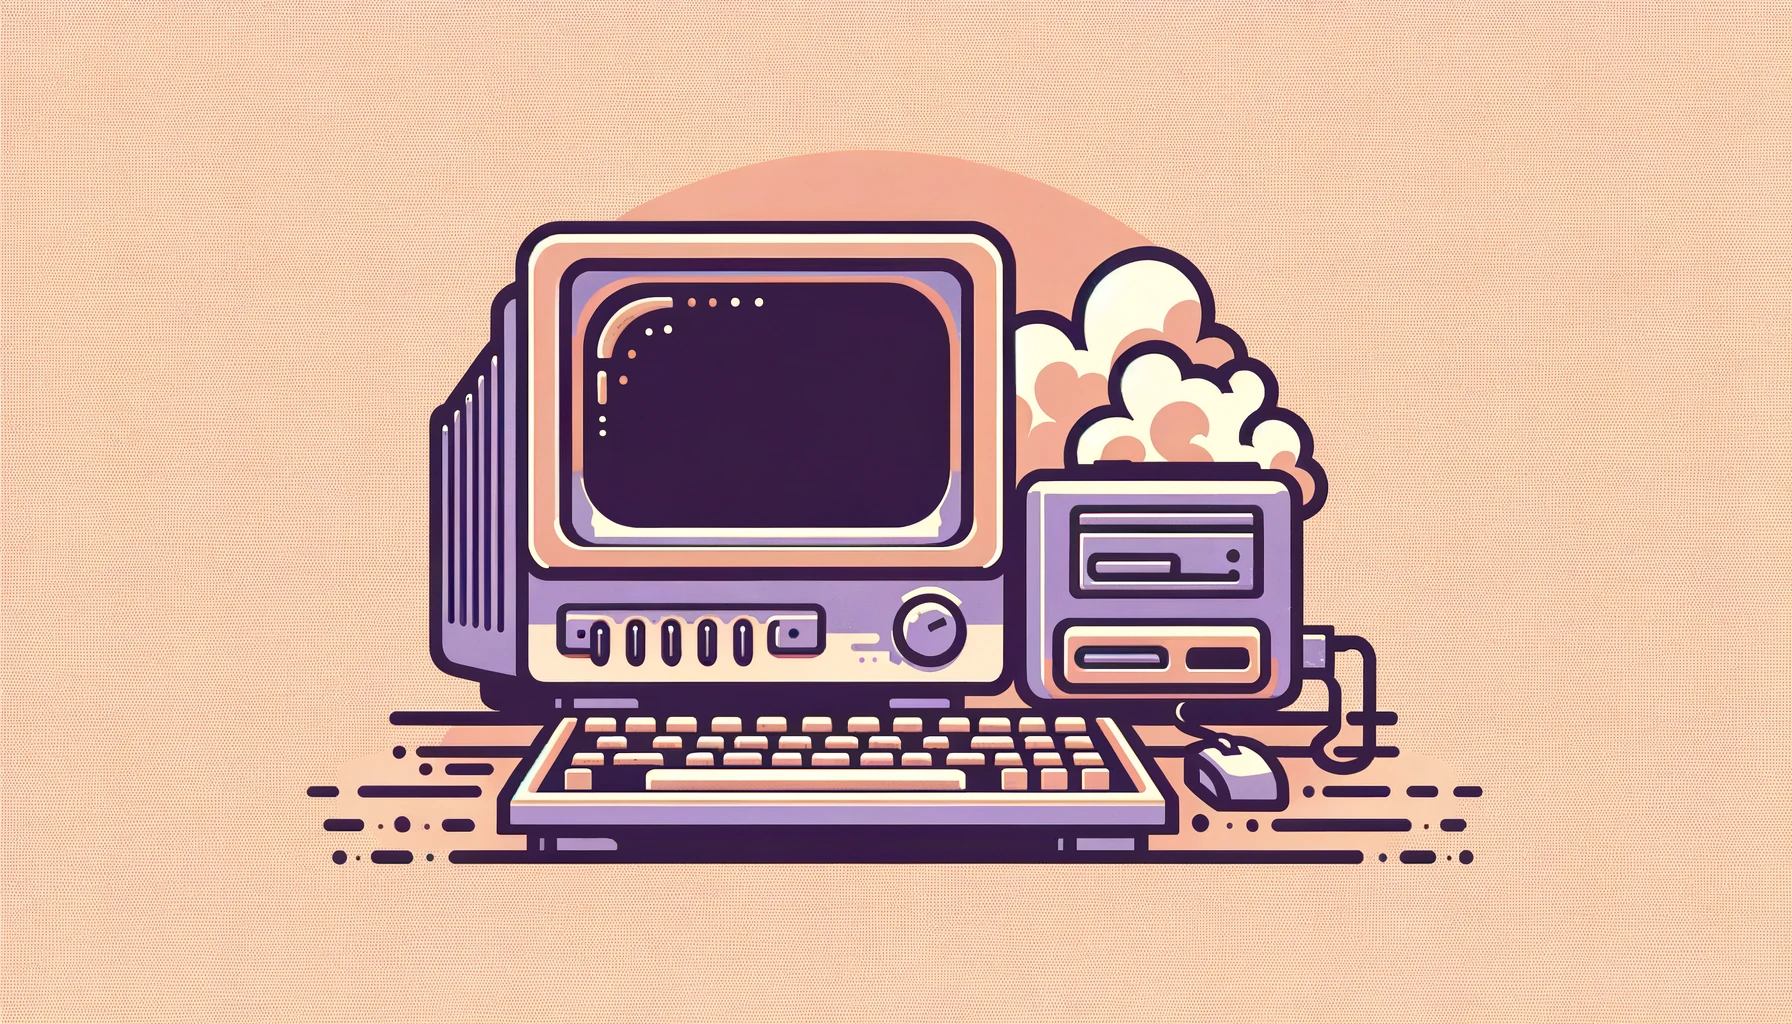
\includegraphics[width=.35\textwidth]{figures/ccomp.png}
\end{figure}

\textbf{On a quantum computer}
\begin{itemize}[noitemsep]
\item[\footnotesize\faCircle] $0.0721\,\,\mu \text{s}$ to find the jack of clubs;
\item[\footnotesize\faCircle] $0.001$ seconds to find the passcode;
\item[\footnotesize\faCircle] $100$ seconds to find the Cobra antidote.
\end{itemize}
\begin{figure}
    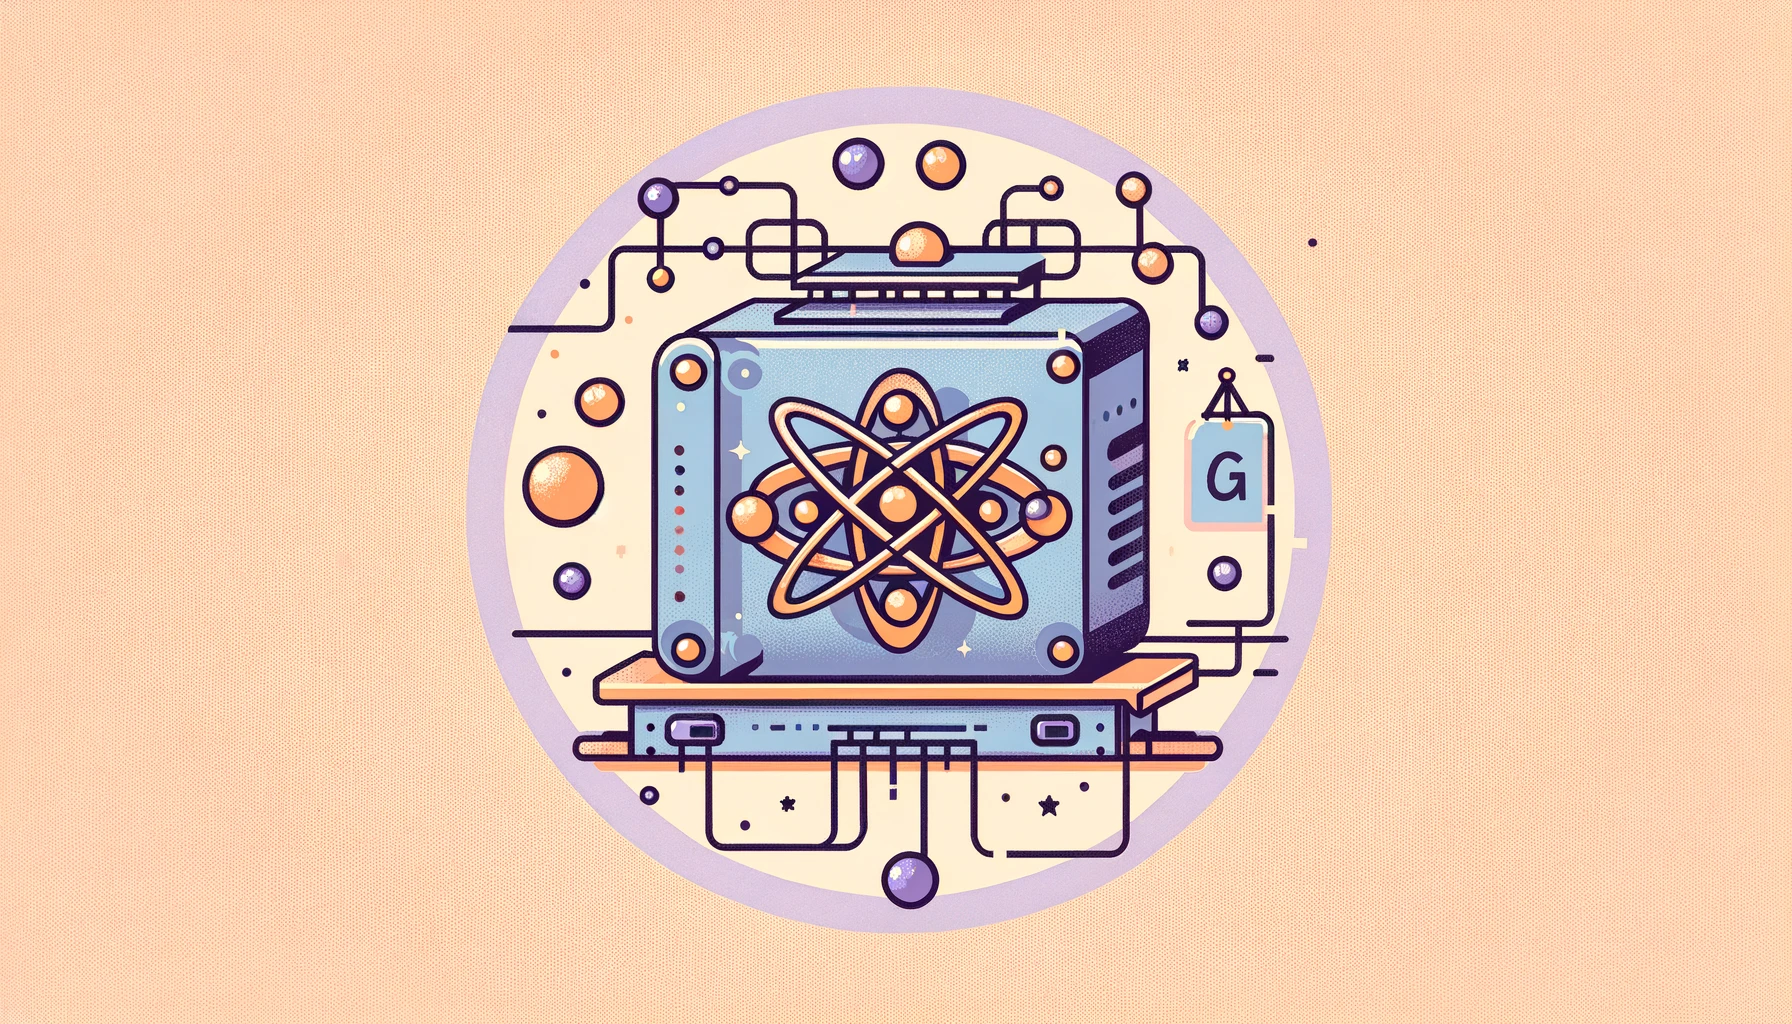
\includegraphics[width=.35\textwidth]{figures/qcomp.png}
\end{figure}
\end{multicols}
\begin{tcolorbox}[colback=red!15]
The Grover algorithm solves this kind of search with a number of algorithmic calls 
proportional to $\sqrt{N}$, where $N$ is the dimension of the search space.
\end{tcolorbox}
\end{frame}


\begin{frame}{The Grover algorithm}
The key steps of the Grover algorithm:

\begin{itemize}[noitemsep]
\item[1.] prepare a system of $N$ qubits into a maximally superposed state;
\item[2.] prepare an ancilla qubit into the $\ket{-}$ state;
\item[3.] apply an oracle operator $U_f$ which can mark the correct solution;
\item[4.] apply a diffusion operator $U_s$ which amplifies the correct solution;
\item[5.] repeat 3. and 4. for the optimal number of times.
\end{itemize}
\pause

In terms of quantum circuit:
\begin{figure}
    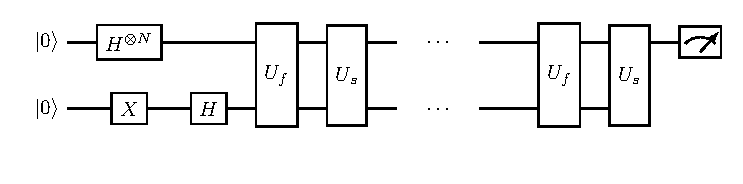
\includegraphics[width=.9\textwidth]{figures/grover-circ.pdf}
\end{figure}
\end{frame}

\begin{frame}{step 1 and 2: the state preparation}
Lets consider $2^N$ elements composing our search space. \pause

We can encode them into the amplitudes of a quantum state of $N$ qubits: 

$$ 
\begin{bmatrix}
\text{item}_1 \\
\text{item}_2 \\
\dots \\
\text{item}_{2^N}
\end{bmatrix} \qquad \to \qquad 
\ket{\psi} = \begin{bmatrix}
\psi_{00 \dots 0} \\
\psi_{00 \dots 1}  \\
\dots \\
\psi_{11 \dots 1}
\end{bmatrix}  
\equiv 
\begin{bmatrix}
x_0 \\
x_1  \\
\dots \\
x_{2^N-1}
\end{bmatrix} . 
$$
\pause 


In total, we will use $N$ qubits of the system and 
one ancilla. Then, the full quantum state will be $\ket{\psi}_N \ket{a}$. \pause

The first step of the algorithm is the state preparation into the following superposed state:
\begin{multicols}{2}
$$ H^{\otimes N + 1} \ket{0}_N \ket{1} = \biggl[ \frac{1}{2^{N/2}}\sum_{i=0}^{2^N - 1} \ket{x_i} \biggr] \otimes \ket{-}. $$

\begin{figure}
   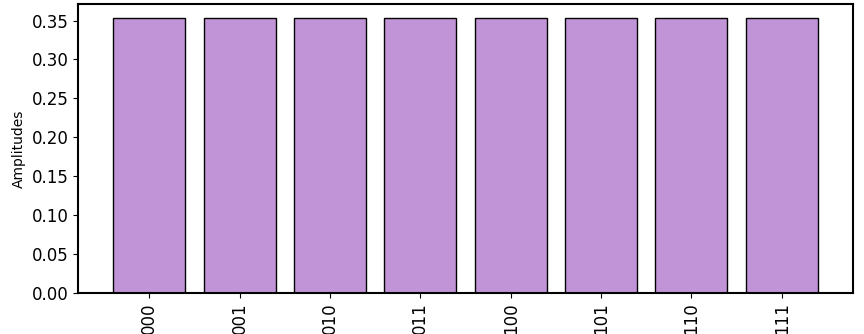
\includegraphics[width=0.45\textwidth]{figures/state1.png}
\end{figure}
\end{multicols}

\end{frame}

\begin{frame}{Step 3: the oracle $U_f$}
We consider now a function $f:\{0,1\}^N \to \{0,1\}.$ whose goal is to mark the correct 
solution:
$$ 
f(x) = \begin{cases}
1 \qquad \text{if\,\,correct}, \\
0 \qquad \text{otherwise}.
\end{cases} $$
This function is typically embedded into a quantum oracle $U_f$ which is able to 
recognize the solution for us. It's important to underline that even if the oracle 
can detect the solution, may don't know it's exact value.

The oracle marks the solution (one of the amplitudes) by flipping its sign thanks to
a phase-kickback procedure.

\begin{multicols}{2}
$$ U_f \ket{x}\ket{-} = (-1)^{f(x)}\ket{x}\ket{-}. $$

This can be done using a multi-controlled operation which triggers the kickback only 
when the system state corresponds to the target one.

\begin{figure}
   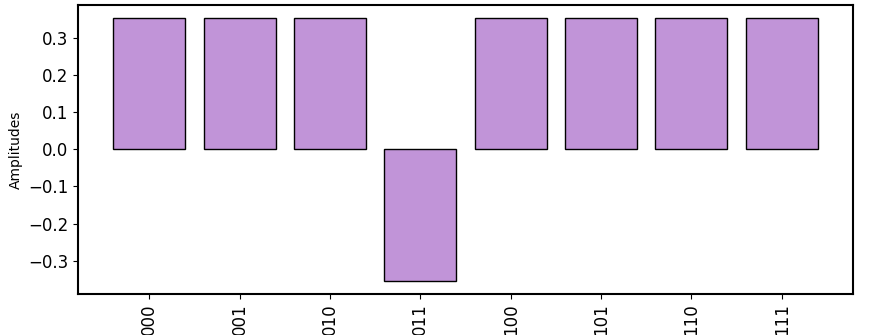
\includegraphics[width=0.5\textwidth]{figures/state2.png}
\end{figure}
\end{multicols}

\end{frame}

\begin{frame}{Step 4: the diffusion operator $U_s$}

\end{frame}

\begin{frame}
\centering
\Huge Let's code!
\begin{figure}
   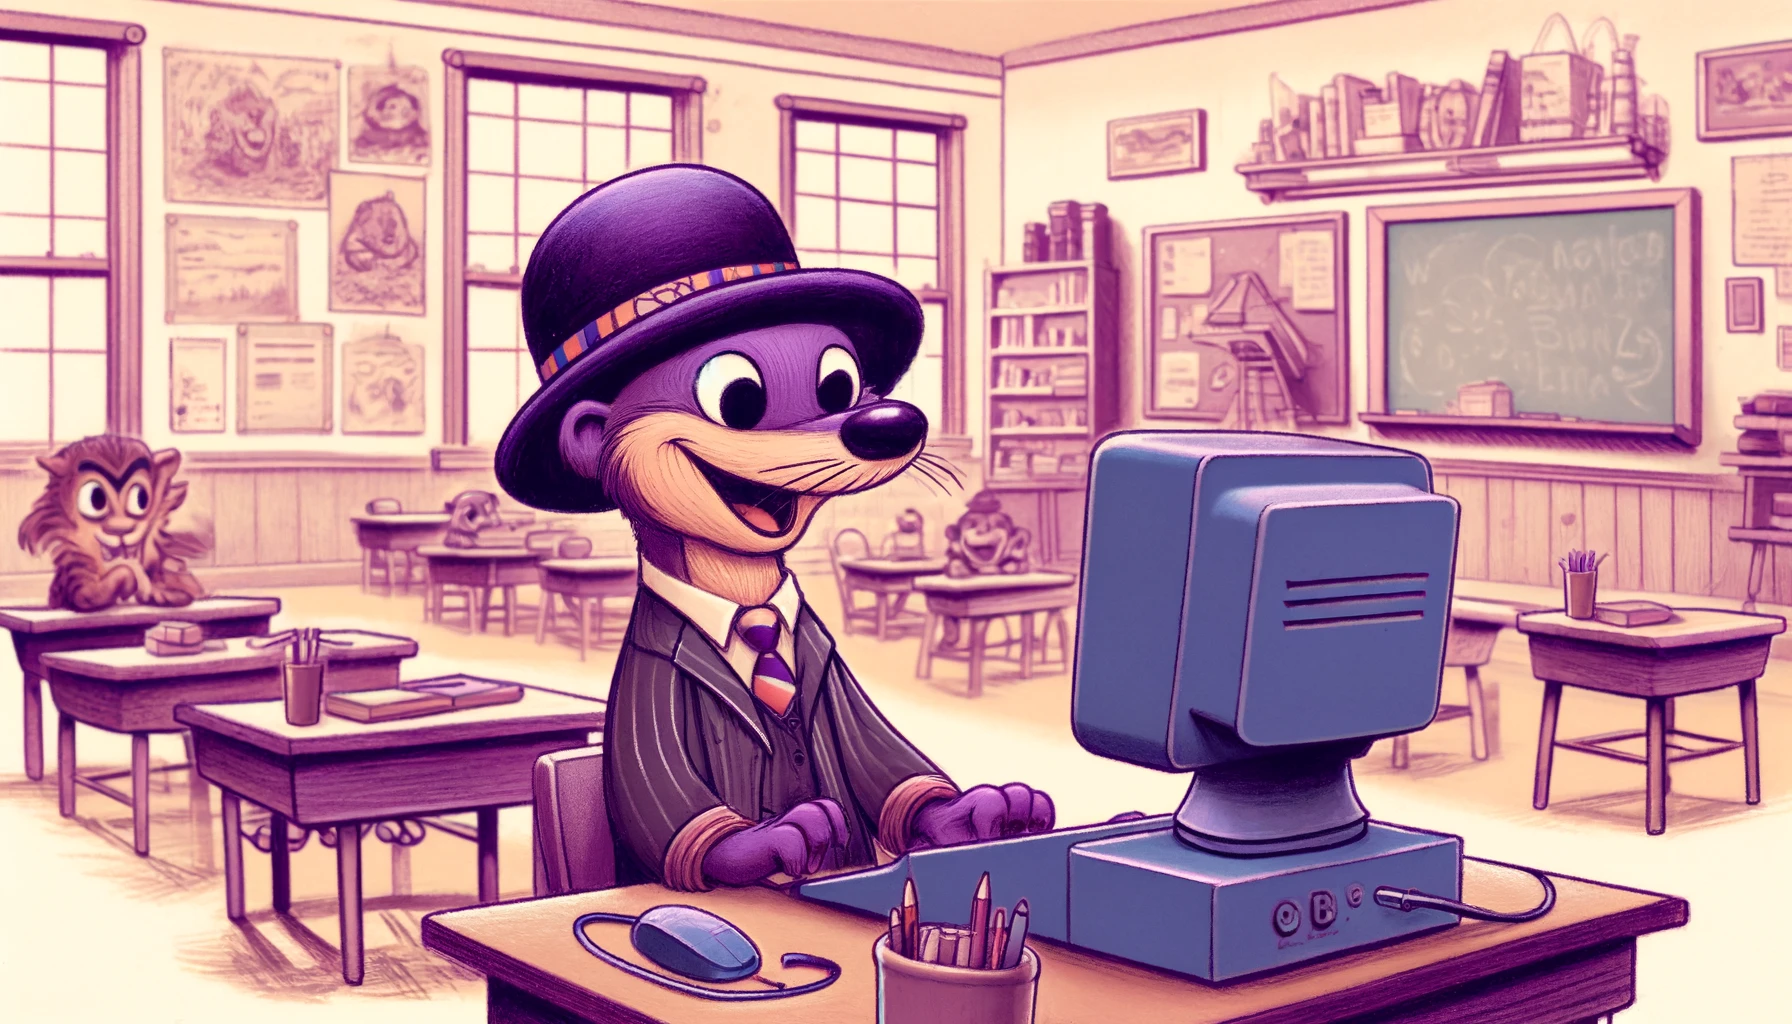
\includegraphics[width=0.7\textwidth]{figures/hands_on.png}
\end{figure}
\end{frame}

\end{document}
